


\setlength{\columnsep}{15pt}%
\setlength{\intextsep}{0pt plus 0pt minus 0pt}


\setlength{\parindent}{\myindent}
% \setlength{\parskip}{\myparskip}

 \vspace*{-10pt}

\subsubsection{Motivation}
\begin{wrapfigure}{r}{140pt}
    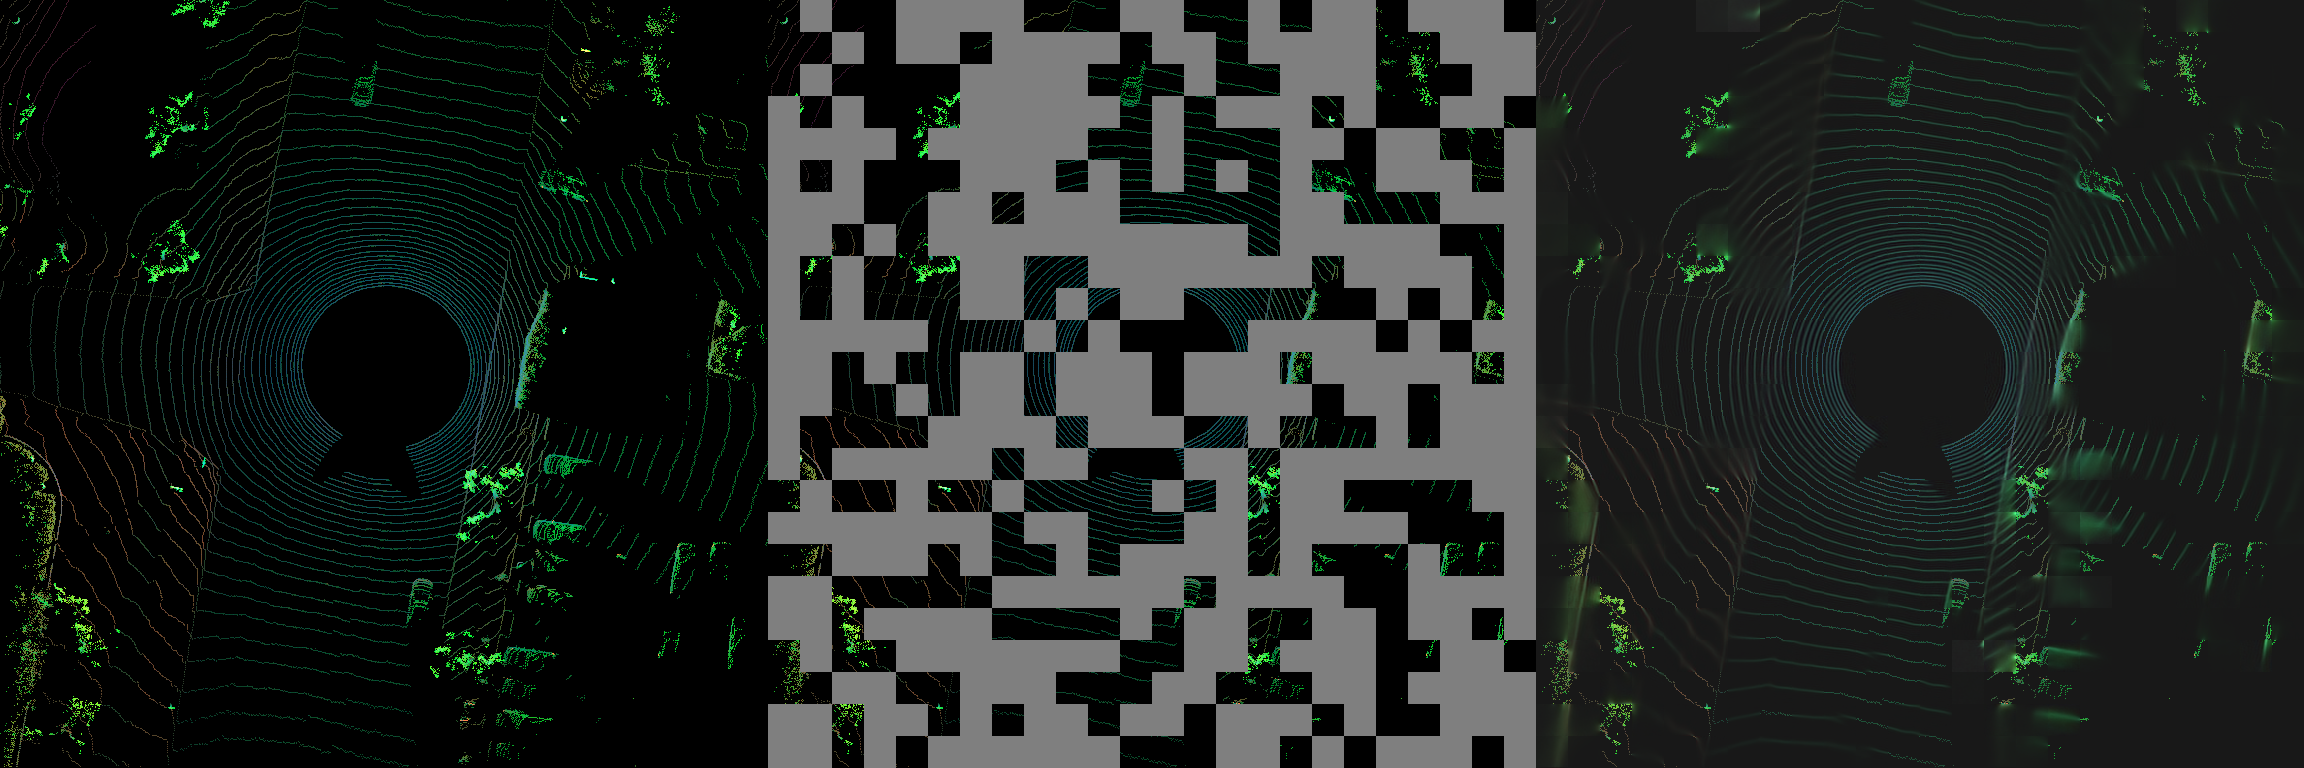
\includegraphics[width=420pt, angle=270]{pic/Hiera-Waymo.png}
    \mainfont\fontsize{9pt}{9pt}\selectfont\caption{ \mainfont\fontsize{9pt}{9pt}\selectfont Masked Autoencoding 
    (MAE) of Bird's Eye View Point Cloud Representation on Waymo Open Perception Dataset. The top shows the input, the middle the masked input and the bottom the 
    reconstruction.}
    \label{fig:mae_img}
    \end{wrapfigure}
    I am interested in computer vision and machine learning (ML) with a focus on perception and scene representation. I am particularly interested in self-supervised and semi-supervised learning techniques since they are important for real-world application with limited annotation budget. My prior research during my work at Research Center for Information Technology (FZI) under Dr. Ömer Sahin Tas and during my master’s thesis under Prof. Christoph Stiller touched on self-supervised learning using masked image modeling, 2D and 3D object detection on camera and lidar input as well as multimodal fusion. I wish to earn a Ph.D. in the field of computer vision and machine learning.

    I focused on computational mechanics in my bachelors where I obtained my fundamental understanding of tensor algebra, tensor analysis as well as optimization. In my bachelor’s thesis supervised by Prof. Thomas Böhlke I researched algorithms to generate higher order irreducible tensor representations in the context of mechanical texture development. I delved into the field of computer vision and machine learning with the exceptional course on Machine Vision by Dr. Martin Lauer. There I immediately recognized the high transferability of the mathematical methods from continuum mechanics and was inspired to pursue a career in the field.

    Motivated by the course on Machine Vision I applied for the internship at SICK AG, where I worked on the embedded application layer of a smart 3D-ToF Camera, used to detect obstacles in indoor scenes using classical ML methods. In many discussions the lack of labeled point cloud data as well as the difficulty to adapt to new domains using off-the-shelf detectors were mentioned as the reason for the slow implementation of deep learning. This emphasizes importance of self-supervised and unsupervised learning techniques. During my internship and time as a working student, I developed my skills as a software engineer and became a more effective team player through hands-on experience and collaboration.

    As part of my Information Technology major field, I had the opportunity to participate in the Data Driven Engineering I/II course series by Dr. Cihan Ates, where I built a strong foundation in machine learning and optimization. With my machine learning research project "Energy Consumption Prediction at High Granularity" I competed at the lecture accompanying project contest, where I placed in the top three. I gained valuable experience in the practical application of classical regression methods and recurrent nueral network approaches such as RNNs and LSTMs. In Data Driven Engineering II, my team and I worked on particle velocity and uncertainty estimation using convolutional autoencoders based on a variance attenuation loss. 



